\chapter{Experimentación}
\label{cap:experimentacion}
En este capitulo desarrollaremos e ilustraremos los diferentes experimentos o pruebas unitarias que se han realizado para la validación del sistema de mapeado dinámico y el sistema de navegación semántica. En primer lugar se realizarán test de mapeado en un entorno doméstico. Con esto comprobaremos que los objetos son eliminados del mapa si desaparecen y como el mapa va cambiando. También haremos pruebas en una estancia de la casa que no aparece en los mapas y comprobaremos como se añade correctamente al mapa. En segundo lugar haremos pruebas de navegación en un entorno doméstico y dinámico y por ultimo expondremos los experimentos llevados a cabo en la RoboCup@Home en el transcurso de la competición.

\section {Mapeado en entorno doméstico}
\label{cap:mapeadodomestico}
En esta primera sección se expondrán los experimentos realizados para validar el proceso por el cual se incluyen o se eliminan los objetos del primer mapa que maneja el servidor de mapas dinámico, el mapa de corto plazo. Estos experimentos se realizarán primero en el simulador Gazebo con el mapa GrannieAnnie, y después en el robot real en el laboratorio.

\subsection {Adición y eliminación de objetos en el mapa de corto plazo en entorno simulado}
\label{sec:add-deleteobjects}

La figura \ref{fig:initserver} fue captada al iniciar el algoritmo. Observamos que la mayor parte del mapa de corto plazo se encuentra en una posición de desconocimiento y que se han ido incluyendo en este las zonas libres, las paredes y la estantería. Los puntos morados y verdes corresponden a la representación de las muestras tomadas por el láser.

\begin{figure}[hbtp]
  \begin{center}
    \subfigure[]{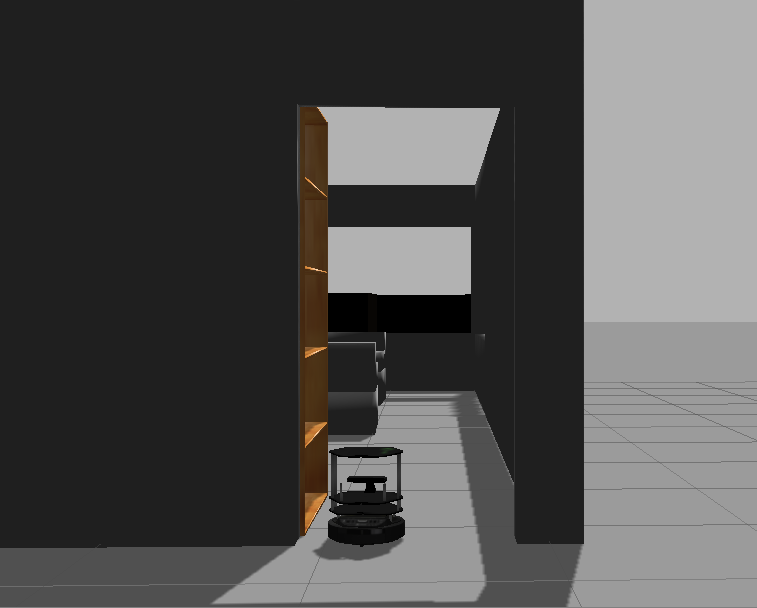
\includegraphics[width=5cm,height=5cm]{img/cap7/incrementmap}}
    \subfigure[]{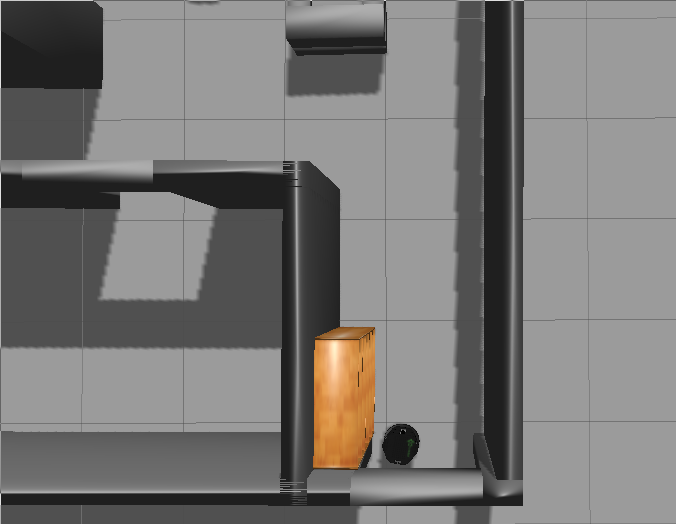
\includegraphics[width=5cm,height=5cm]{img/cap7/incrementmap2}}
    \subfigure[]{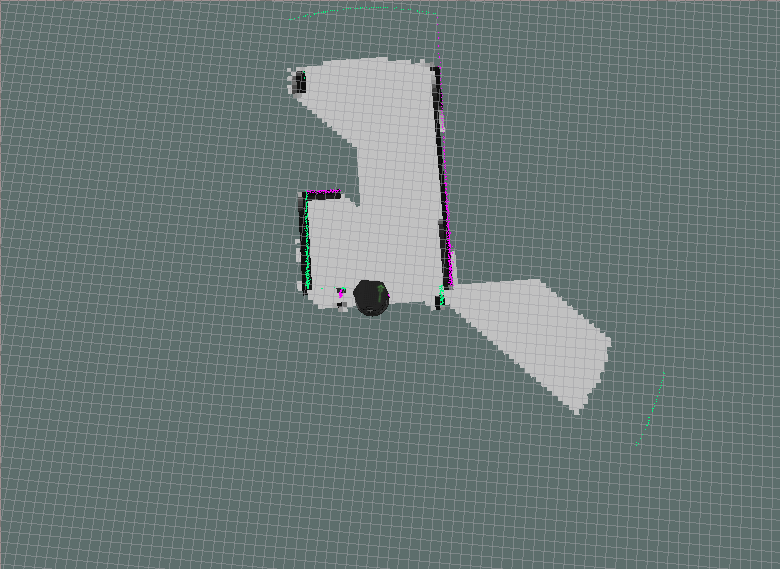
\includegraphics[width=5cm,height=5cm]{img/cap7/incrementmap-rviz}}
  \end{center}
  \caption{Visión del simulador, (a) y (b), y mapa a corto plazo (c).}
  \label{fig:initserver}
\end{figure}

Tras el inicio del algoritmo se añadió un objeto nuevo al escenario. Esto se representa en la figura \ref{fig:includeobject}. Vemos como el objeto ha sido reconocido por el láser, ya que podemos observar su contorno en las marcas de colores verdes y que el algoritmo añade el objeto al mapa y lo sitúa en una posición coherente respecto a la posición que ocupa el objeto en el escenario simulado.

\begin{figure} [hbtp]
  \begin{center}
    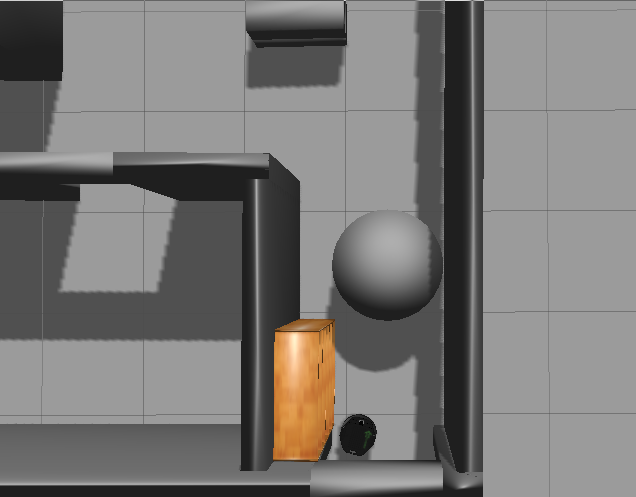
\includegraphics[width=6cm,height=5cm]{img/cap7/incrementmap-object3}
    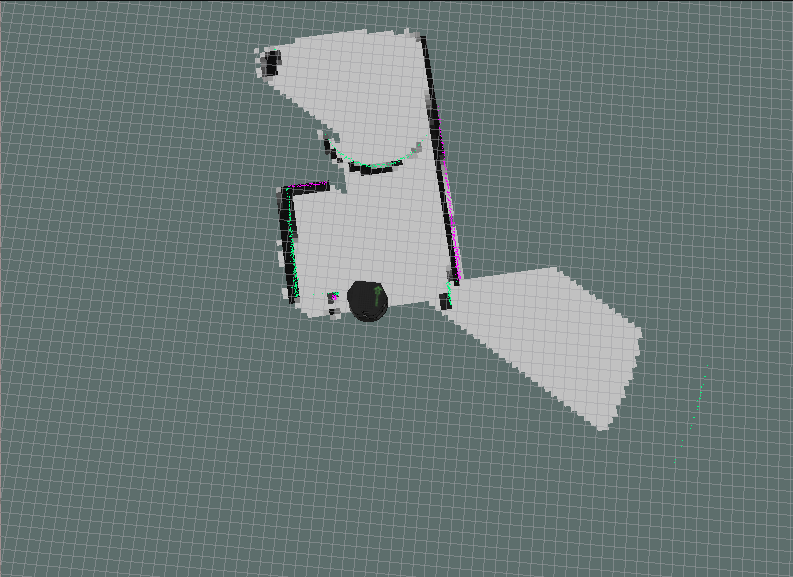
\includegraphics[width=6cm,height=5cm]{img/cap7/incrementmap-object}
  \end{center}
  \caption{Añadimos un objeto al escenario}
  \label{fig:includeobject}
\end{figure}

Una vez que el algoritmo a incluido el objeto en el mapa procedemos a eliminarlo del escenario simulado. Se observa también que las marcas del láser ya no aparecen superpuestas en el mapa. Esto se representa en la figura  \ref{fig:deleteobject}. Vemos como el algoritmo ha comenzado a borrar el objeto, por lo que el valor de las celdas que estaban ocupadas por el objeto ahora es mucho menor.

\begin{figure}[hbtp]
  \begin{center}
    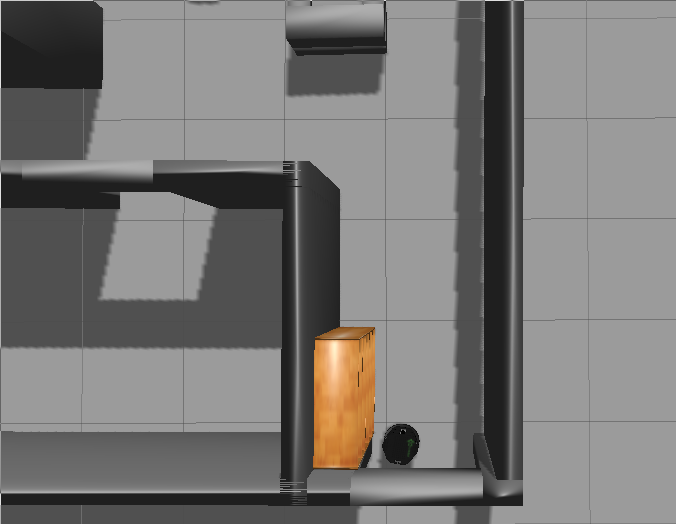
\includegraphics[width=6cm,height=5cm]{img/cap7/incrementmap2}
    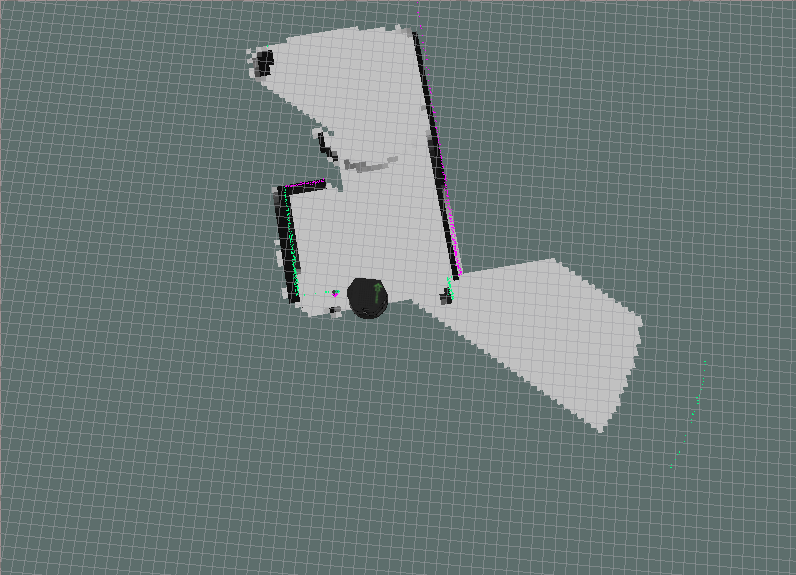
\includegraphics[width=6cm,height=5cm]{img/cap7/incrementmap-object2}
  \end{center}
  \caption{Eliminamos un objeto del escenario}
  \label{fig:deleteobject}
\end{figure}

\subsection {Adición y eliminación de objetos en el mapa de corto plazo en entorno real}
\label{sec:add-deleteobjectsreal}

GRAFICA ADICION: RELACION VALOR VARIABLE / TIEMPO
GRAFICA BORRADO: RELACION VALOR VARIABLE / TIEMPO

\subsection {Adición y eliminación de objetos en el mapa de largo plazo en entorno simulado}
\label{sec:add-deleteobjectslong}
En el siguiente experimento probaremos el añadido y borrado de objetos en el mapa de largo plazo. Para ello realizamos el mismo experimento que en la sección anterior aunque ahora el objeto en el camino del robot es un sofá. Observamos en la figura \ref{fig:addobjectlongmap} como se encuentra el nuevo objeto y al cabo de un tiempo lo añade al mapa de largo plazo. 
\begin{figure}[hbtp]
  \begin{center}
    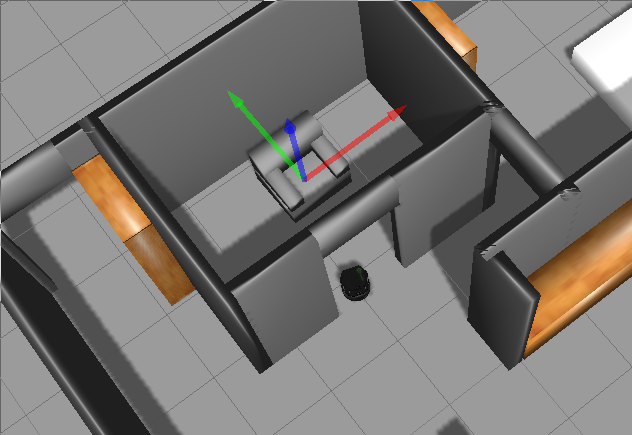
\includegraphics[width=10cm,height=6cm]{img/cap7/addingobject-gazebo}
    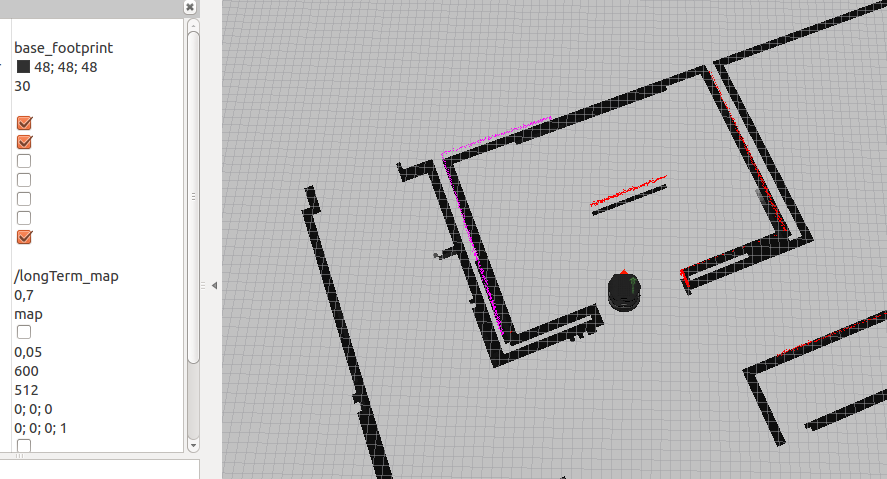
\includegraphics[width=10cm,height=5cm]{img/cap7/addingobject-longmap}
  \end{center}
  \caption{Añadimos un objeto al mapa de largo plazo}
  \label{fig:addobjectlongmap}
\end{figure}
En la figura \ref{fig:deleteobjectlongmap} el objeto ha sido eliminado del entorno simulado y el algoritmo comienza a borrarlo también del mapa de largo plazo. Observamos como ha disminuido el valor de las celdas ocupadas anteriormente por el sofá.

\begin{figure}[hbtp]
  \begin{center}
    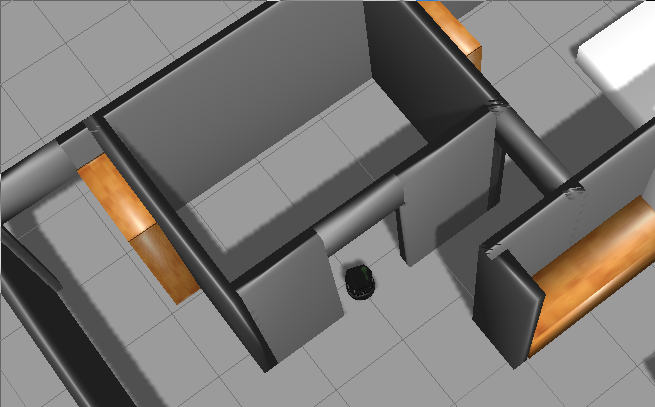
\includegraphics[width=10cm,height=5cm]{img/cap7/deletingobject-gazebo}
    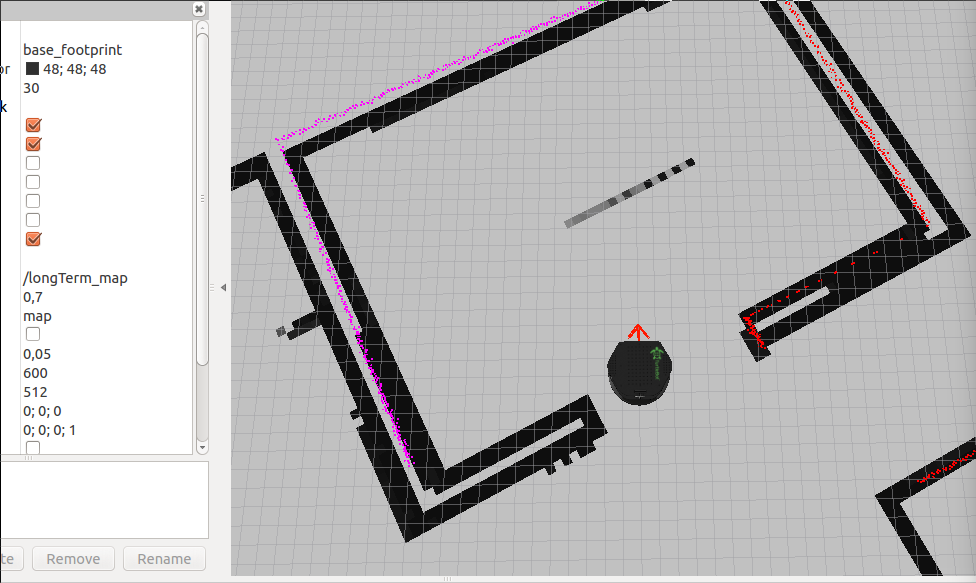
\includegraphics[width=10cm,height=5cm]{img/cap7/deletingobject-longmap}
  \end{center}
  \caption{Borramos un objeto del mapa de largo plazo}
  \label{fig:deleteobjectlongmap}
\end{figure}

GRAFICA BORRADO: RELACION VALOR VARIABLE / TIEMPO

\subsection {Mapeado de zonas desconocidas.}
Para este experimento se ha extendido ligeramente el mapa simulado, de tal forma que se han añadido unos pasillos nuevos a la derecha del escenario, como vemos en la figura \ref{fig:grannieAnne-ext}. Esta zona no vamos a incluirla previamente en el mapa estático ni en el mapa de largo plazo y queremos comprobar si el sistema es capaz de añadir una zona nueva al mapa y localizarse correctamente. El mapa estático usado es el mismo que el mostrado en la figura \ref{fig:mapaestatico}.
\begin{figure}[H]
  \begin{center}
    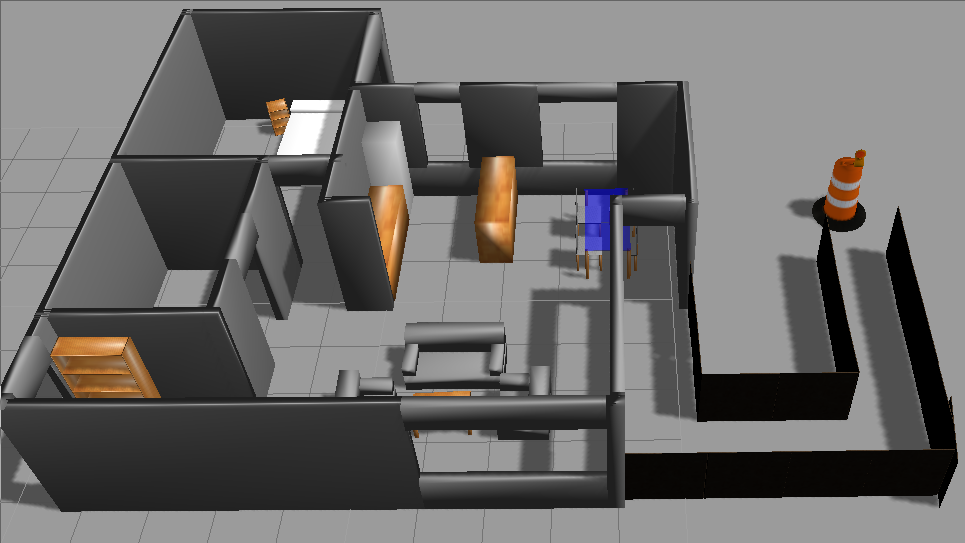
\includegraphics[width=12cm,height=7cm]{img/cap7/grannieAnne-ext}
  \end{center}
  \caption{Escenario extendido}
  \label{fig:grannieAnne-ext}
\end{figure}

\begin{figure}[hbtp]
  \begin{center}
    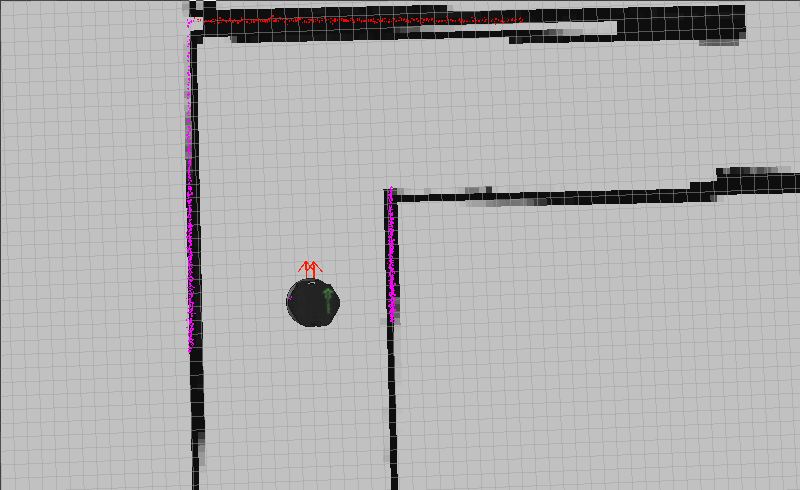
\includegraphics[width=10cm,height=6cm]{img/cap7/localization-ext}
  \end{center}
  \caption{Detalle de la localización}
  \label{fig:localization-ext}
\end{figure}

\begin{figure}[hbtp]
  \begin{center}
    \subfigure[Mapa total]{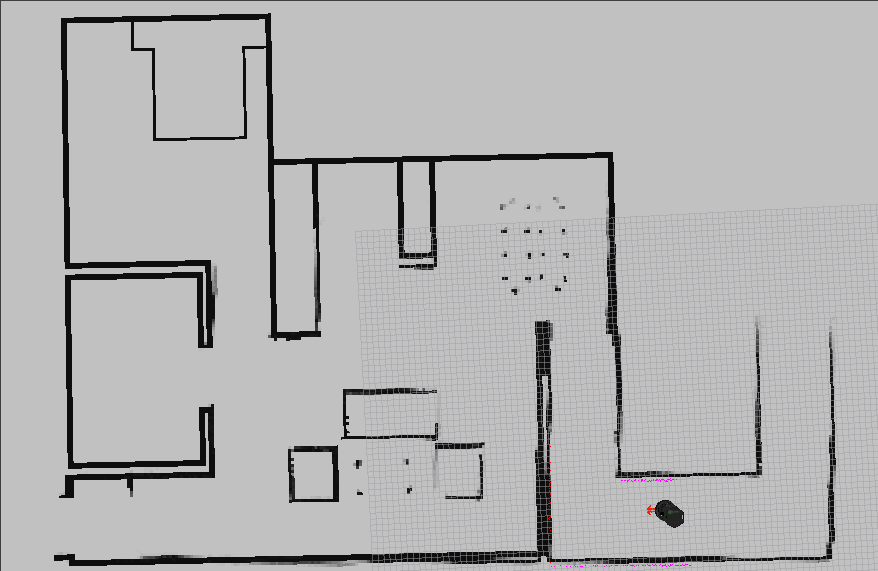
\includegraphics[width=12cm,height=7cm]{img/cap7/map-ext}}
    \subfigure[Mapa de largo plazo]{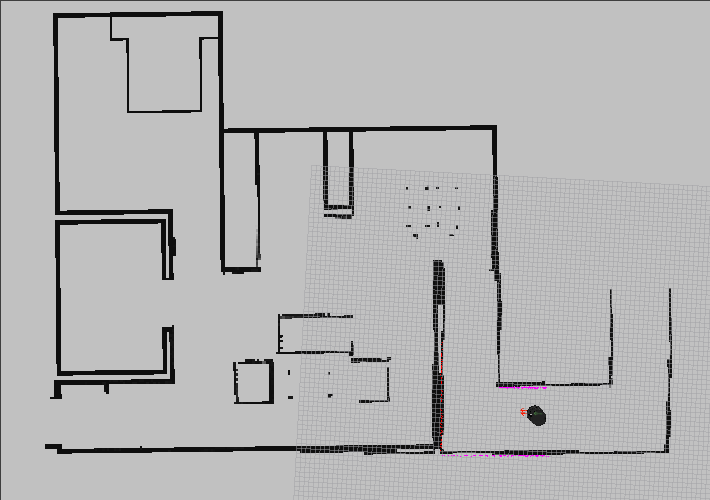
\includegraphics[width=12cm,height=7cm]{img/cap7/longmap-ext}}
    \subfigure[Mapa de corto plazo]{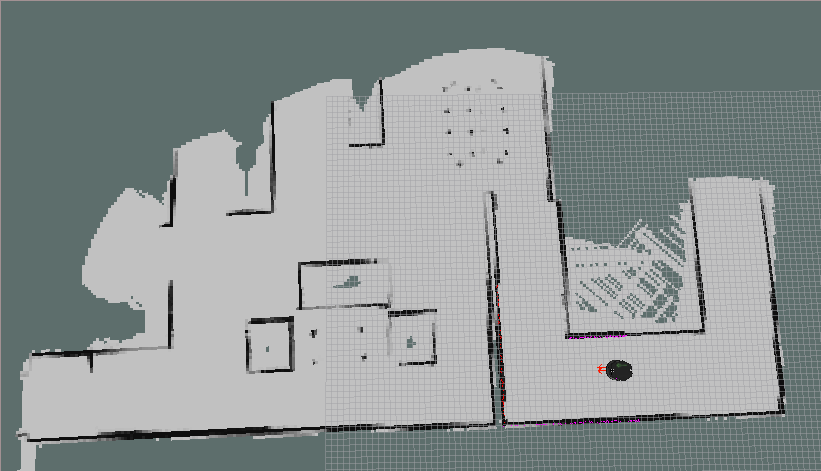
\includegraphics[width=12cm,height=7cm]{img/cap7/shortmap-ext}}
  \end{center}
  \caption{Mapas del escenario extendido}
  \label{fig:maps-ext}
\end{figure}

  Vemos como después de recorrer la parte desconocida del mapa se ha añadido al mapa de largo plazo y también al mapa total, figura \ref{fig:maps-ext}. Observamos en las flechas rojas bajo el robot que la incertidumbre en la posición del robot es mínima, figura \ref{fig:localization-ext}. Comprobamos con este experimento la potencia de esta característica de nuestro sistema, somos capaces de añadir zonas completas al mapa sin necesidad de reiniciar el algoritmo ni de modificar el mapa estático, y seguir completamente localizados.

\subsection {Adición y eliminación de objetos en el mapa de largo plazo en entorno real}
\label{sec:add-deleteobjectslongreal}

\section {Navegación con obstáculos dinámicos}
\label{cap:navegacionconobstaculos}

\section {Experimentación en la Robocup}
\label{cap:experimentacionrobocup}

El día 27 de Junio de 2016 el equipo Gentlebot viajó a Leipzig para participar en la Robocup 2016, en la categoría Home. El equipo lo formábamos 4 personas de la universidad de León y 4 personas de la URJC. En este apartado detallaremos las distintas actividades llevadas a cabo en los días de preparación y en los días de competición. 

El robot con el que participamos en la competición, detallado en el capitulo XXX, fue el RB1. Las pruebas a disputar fueron las siguientes: Navigation, Speech Recognition \& Audio Detection, Person Recognition, Manipulation \& Object Recognition, Following \& Guiding y General Purpose Service Robot y estas pruebas se disputarían en 2 escenarios desconocidos a priori, tanto en dimensiones como en los objetos que contendrían. El sistema de navegación propuesto estaba involucrado en las pruebas de Navigation, Following \& Guiding y General Purpose Service Robot. 

\begin{itemize}
\item \textbf{Día 1.} Una vez nos instalamos y montamos el robot, que para el viaje hubo que desmontar algunas partes, nos dispusimos a medir las dos arenas para crear los mapas estáticos. Los equipos estábamos organizados en turnos para usar los escenarios y así probar los mapas o anotar \textit{waypoints} por los que el robot debiera pasar o alcanzar. Una vez creados los mapas estáticos y hacer que el robot creara los mapas de largo plazo con algunos objetos que había en las arenas, nos dispusimos a retocarlos ligeramente. Al no disponer del robot RB1 físicamente hasta la llegada a la competición no tuvimos en cuenta algunos detalles, como por ejemplo que el robot no podía pasar por debajo de una mesa por ser mucho más alto que el robot kobuki. Esto no tendría por qué haber sido un impedimento, pero los árbitros de la competición situaron mesas muy cercanas a las puertas por las que el robot tendría que entrar en la arena. Esto generaba que la ruta que establecía el nodo \textit{move\_base} cruzaba la mesa y ademas el robot, al tener el láser en la base, no añadía al mapa un objeto de las dimensiones de una mesa, solo añadía las patas. Por esto hubo que añadir a mano algunos objetos al mapa de largo plazo. Tras esto también empezamos a preparar y a ensayar la prueba de Inspección que tienen que pasar todos los robots que tendría lugar al día siguiente.
\item \textbf{Día 2.} En el día 2 se anunció en que arena tendría lugar la inspección y en por qué puerta se entraría a la inspección, por lo que cogimos un punto de referencia en esa puerta para establecerlo como punto de inicio del robot dentro del mapa. También comenzamos a preparar la prueba de navegación que tendría lugar al día siguiente y que involucraba las 2 arenas, ya que se haría en 3 tandas y se iría alternando de arena. La inspección consistía en entrar en la arena y acercarse a un mueble, este era el \textit{waypoint 1}. Entre el mueble y el robot se colocaba un árbitro al que el robot no podía tocar. Una vez el robot comenzaba a sortear al arbitro este se retiraba. Al llegar al \textit{waypoint 2} el robot se paraba y esperaba que un arbitro se enseñara un código QR que el indicaba que debía continuar. Tras esto el robot cruzaba una puerta y si todo estaba correcto los árbitros probaban el botón de emergencia, parando el robot y finalizando así la prueba. El resto del día anotamos los diferentes \textit{waypoints} de la prueba de navegación, ensayamos en las arenas con estos waypoints y preparamos otras pruebas del día 3, como la prueba de Speech Recognition \& Audio Detection.
\item \textbf{Día 3.} El comienzo del día 3 nos deparó una pequeña sorpresa. No sabíamos, o no teníamos del todo claro, si la puerta de la arena iba a estar cerrada o abierta al comenzar la prueba, por lo que no teníamos del todo claro cuando se debía lanzar el algoritmo de navegación. Los jueces nos aclararon que se debía lanzar todos los algoritmos y en ese momento llamar a la puerta y desde dentro un juez nos abriría. Este primer escollo nos costó no puntuar en la primera manga de la prueba de navegación, aunque pudimos solventarlo antes de las siguientes tandas. En la segunda tanda, el robot pasó correctamente por la puerta y comenzó a navegar por la casa, sorteando una mesa primero, a un juez después y cambió de ruta cuando una puerta se cerró cuando estaba a punto de pasar por ella. Una silla de finas patas metálicas arruinó nuestra prueba cuando la pusieron entre el robot y la puerta de la habitación. 

En la tercera tanda nos esperaba el más difícil todavía, sortear un vaso de 5cm de altura, que aunque RB1 pudo recalcular bien su ruta para intentar esquivarlo no pudo evitar tocarlo ligeramente para más tarde volver a toparse con una silla en el camino. 

Las pruebas de Speech Recognition \& Audio Detection salieron muy bien, siendo uno de los equipos que mayor puntuación.

\item \textbf{Día 4.} El cuarto día fue nuestro último día como participantes en la RoboCup@Home ya que no obtuvimos los suficientes puntos para clasificarnos para la siguiente fase. La pruebas en las que participamos en este día fueron: Manipulation \& Object Recognition y Following \& Guiding. En la primera no obtuvimos unos buenos resultados ya que no fuimos capaces de reconocer los objetos que se nos presentaron y en la segunda tampoco, ya que no fuimos capaces de reconocer correctamente al árbitro para después seguirle. Esta prueba hubiera explotado la parte del algoritmo en la que se van añadiendo zonas nuevas al mapa ya que consistía en seguir a un árbitro por fuera de las arenas, una zona no mapeada, y luego devolverle a casa.
\end{itemize}


